\chapter[King Harald Goes West-Over-Seas]{
    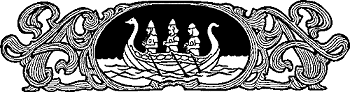
\includegraphics[width=9.3cm]{viking-tales/032}\\
    King Harald Goes West-Over-Seas}

\lettrine{N}{ow} many men hated King Harald. Many a man said:
\vskip2\baselineskip
``Why should he put himself up for king of all of us? He is no better
than I am. Am I not a king's son as well as he? And are not many of us
kings' sons? I will not kneel before him and promise to be his man. I
will not pay him taxes. I will not have his earl sitting over me. The
good old days have gone. This Norway has become a prison. I will go away
and find some other place.''

So hundreds of men sailed away. Some went to France and got land and
lived there. Big Rolf-go-afoot and all his men sailed up the great
French River and won a battle against the French king himself. There was
no way to stop the flashing of his battle-axes but to give him what he
wanted. So the king made Rolf a duke, gave him broad lands and gave him
the king's own daughter for wife. Rolf called his country Normandy, for
old Norway. He ruled it well and was a great lord, and his sons' sons
after him were kings of England.

Other Norsemen went to Ireland and England and Scotland. They drew up
their boats on the river banks. The people ran away before them and
gathered into great armies that marched back to meet the vikings in
battle. Sometimes the Norsemen lost, but oftener they won, so that they
got land and lived in those countries. Their houses sat in these strange
lands like warriors' camps, and the Norsemen went among their new
neighbors with hanging swords and spears in hand, ever ready for fight.

There are many islands north of Scotland. They are called the Orkneys
and the Shetlands. They have many good harbors for ships. They are
little and rocky and bare of trees. Wild sea-birds scream around them.
On some of them a man can stand in the middle and see the ocean all
about him. Now the vikings sailed to these islands and were pleased.

\begin{figure}[ht]
    \centering
    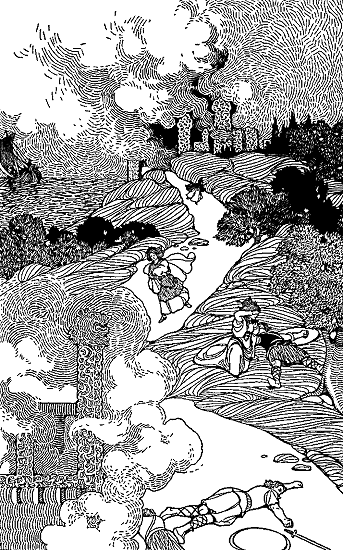
\includegraphics[width=9.1cm]{viking-tales/033}
    \caption{``In Norway they left burning houses and weeping women''}
\end{figure}

``It is like being always in a boat,'' they said. ``This shall be our
home.''

So it went until all the lands round about were covered with vikings.
Norse carved and painted houses brightened the hillsides. Viking ships
sailed all the seas and made harbor in every river. Norsemen's thralls
plowed the soil and planted crops and herded cattle, and gold flowed
into their masters' treasure-chests. Norse warriors walked up and down
the land, and no man dared to say them nay.

These men did not forget Norway. In the summers they sailed back there
and harried the coast. They took gold and grain and beautiful cloth back
to their homes. In Norway they left burning houses and weeping women.

Every summer King Harald had out his ships and men and hunted these
vikings. There are many little islands about Norway. They have crags and
caves and deep woods. Here the vikings hid when they saw King Harald's
ships coming. But Harald ran his boat into every creek and fiord and
hunted in every cave and through all the woods and among the crags. He
caught many men, but most of them got away and went home laughing at
Harald. Then they came back the next summer and did the same deeds over
again. At last King Harald said:

``There is but one thing to do. I must sail to these western islands and
whip these robbers in their own homes.''

So he went with a great number of ships. He found as brave men as he had
brought from Norway. These vikings had brought their old courage to
their new homes. King Harald's fine ships were scarred by viking stones
and scorched by viking fire. The shields of Harald's warriors had dents
from viking blows. Many of those men carried viking scars all their
lives. And many of King Harald's warriors walked the long, hard road to
Valhalla, and feasted there with some of these very vikings that had
died in King Harald's battles. But after many hard fights on land and
sea, after many men had died and many had fled away to other lands, King
Harald won, and he made the men that were yet in the islands take the
oath, and he left his earls to rule over them. Then he went back to
Norway.

``He has done more than he vowed to do,'' people said. ``He has not only
whipped the vikings, but he has got a new kingdom west-over-seas.''

Then they talked of that dream that his mother had.

``King Harald was that great tree,'' they said. ``The trunk was red with
the blood of his many battles, but higher up the limbs were fair and
green like this good time of peace. The topmost branches were white
because Harald will live to be an old man. Just as that tree spread out
until all of Norway was in its shade, and even more lands, so Harald is
king of all this country and of the western islands. The many branches
of that tree are the many sons of Harald, who shall be earls and kings
in Norway, and their sons after them, for hundreds of years.''
